\centerline{\bf \huge 9 класс}
\centerline{\bf \huge Решения}

\problem{9.1}
Дан квадратный трёхчлен $f(x)$. Известно, что линейная функция $y= f(x+1)-f(x)$ обращается в ноль только при $x=2024$. При каком значении аргумента обращается в ноль функция $y=f(x-1)-f(x)$ ?

\textit{Ответ: $x=2025$.}

\textit{Решение.} 
Обозначим линейную функцию $f(x+1)-f(x)$ за $g(x)$. По условию имеем $g(2024)=0$. Заметим, что функция $h(x)=f(x-1)-f(x)=-g(x-1)$. Значит, $h(x)=0$, тогда и только тогда, когда $-g(x-1)=0$, что в свою очередь равносильно $x-1=2024$, то есть $x=2025$.

\problem{9.2}
На доске написаны четыре числа: $2,3,4$ и 9. За один шаг можно выбрать любые три из них, первое умножить на 2 , второе --- на 4 , а третье --- на 6 (при этом три старых числа стирают, а на их место записывают три новых). Можно ли через несколько шагов получить на доске четыре равных числа?

\textit{Ответ: Нельзя.}

\textit{Решение.}
Произведение изначальных чисел на доске равнялось $2^3 \cdot 3^3$, а после каждой операции оно увеличивается в $2 \cdot 4 \cdot 6=2^4 \cdot 3^1$ раз, поэтому после $n$ таких операций произведение чисел на доске будет равно $2^{3+4 n} \cdot 3^{3+n}$. Если после нескольких таких операций получились четыре равных числа, то их произведение имеет вид $2^{4 x} \cdot 3^{4 y}$, для натуральных $x$ и $y$. Но число $3+4 n$ не может равняться $4 x$, так как не делится на 4 , получаем противоречие.

\problem{9.3}
Найдите значение суммы

$$
\begin{gathered}
S=\left(1^2+1 \cdot 3+3^2\right)+\left(3^2+3 \cdot 5+5^2\right)+\left(5^2+5 \cdot 7+7^2\right)+\cdots \\
+\left(97^2+97 \cdot 99+99^2\right)+\left(99^2+99 \cdot 101+101^2\right)
\end{gathered}
$$

\textit{Ответ: $\frac{101^3-1^3}{2}=515150$.}

\textit{Решение.}
Заметим, что $a^2+a b+b^2=\frac{b^3-a^3}{b-a}$.

Тогда $S=\frac{3^3-1^3}{3-1}+\frac{5^3-3^3}{5-3}+\ldots+\frac{101^3-99^3}{101-99}=\frac{101^3-1^3}{2}=515150$.


\problem{9.4}
В треугольнике $A B C$ медиана $B M$ образует со стороной $B C$ прямой угол. На стороне $A B$ отмечена точка $X$ так, что $\angle B M C=\angle B M X$. Найдите, чему равно отношение $A X: X B$.

\textit{Ответ: 2:1.}

\textit{Решение.}
Отметим середину отрезка $C M$ - точку $N$. Отрезок $B N$ является медианой, проведённой к гипотенузе, прямоугольного треугольника $B M C$, поэтому $B N=M N$. Тогда треугольник $B M N$ равнобедренный, откуда $\angle N B M=\angle B M C=\angle B M X$. Значит, $B N \| M X$. Наконец, по теореме Фалеса $A X: X B=A M: M N=2: 1$.

\begin{figure}[h]
    \centering
    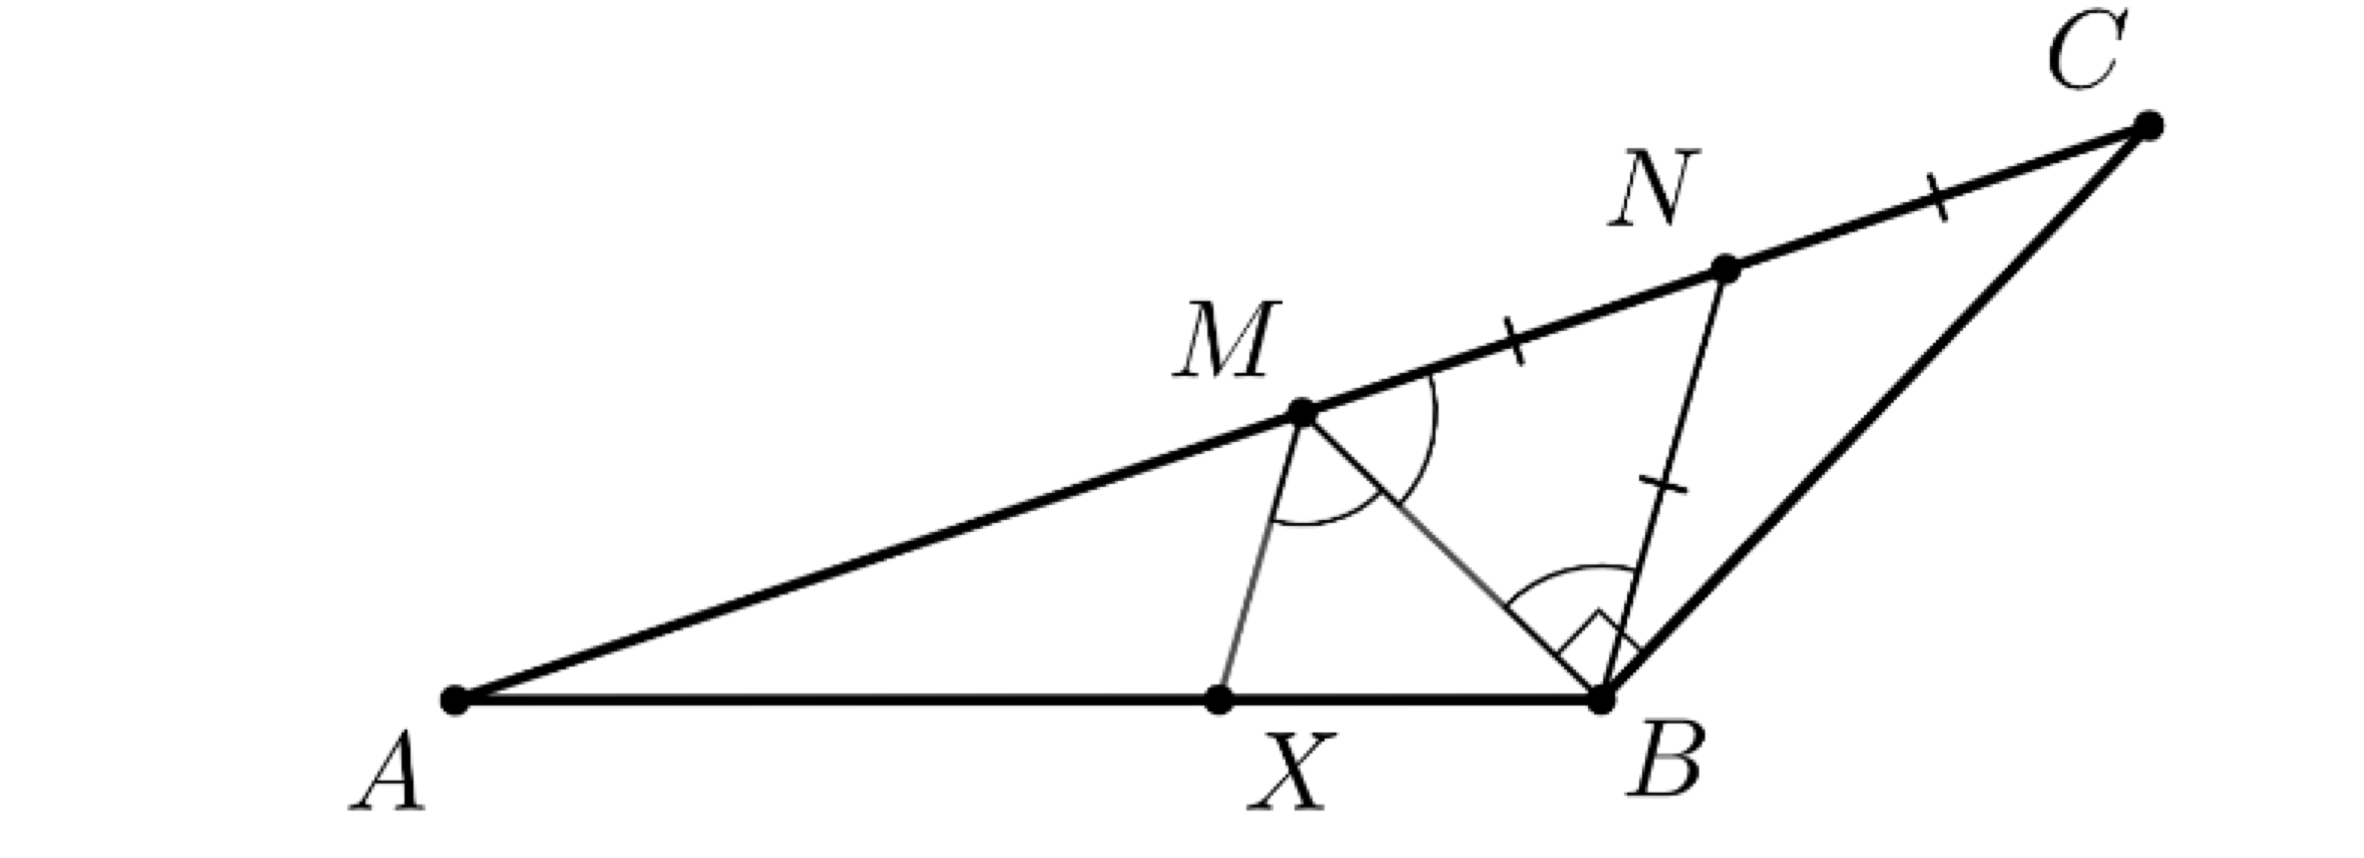
\includegraphics[width=0.5\linewidth]{ЭлМШ 2025-2026//III блок//10//Тренировки//III//Решения/9.3.4.png}
    \caption{}
    \label{fig:placeholder}
\end{figure}

\problem{9.5}
На столе лежат $90$ карточек с числами от $1$ до $90$. Герман и Вова играют в следующую игру. Ходят по очереди. За один ход можно взять со стола любую карточку. Игра заканчивается, когда на столе останется две карточки. Вова выигрывает, если числа на оставшихся карточках отличаются ровно на $10$ . Иначе выигрывает Герман. Кто выигрывает при правильной игре, если начинает Герман?

Ответ: Герман.

Решение. Опишем стратегию Германа. Пусть он выделит следующие карточки: с числами от 11 до 20 (включительно), от 31 до 40 , от 51 до 60 и от 71 до 80 . Выделенных карточек 40 . Невыделенные карточки разобьются на 5 групп по 10 карточек (с числами от 1 до 10 , от 21 до 30 , от 41 до 50 , от 61 до 70 и от 81 до 90 ), причем если две невыделенные карточки находятся в одной группе, то числа на них отличаются не больше чем на 9, а если в разных, то не меньше чем на 11. Всего в игре каждый игрок сделает по 44 хода. Поэтому за свои первые 40 ходов Герман должен забрать выделенные карточки (это произойдет быстрее, если Вова игрок также заберет какие-то выделенные карточки). Поэтому в конце игры останутся две невыделенные карточки, и числа на них будут отличаться не на 10.